\section{COMPONENTE SERVIDOR}

El componente servidor se ha implementado utilizando el lenguaje PHP (\emph{Hypertext Preprocessor}). Se ha utilizado este lenguaje de programación debido a que es uno de los lenguajes de desarrollo web más utilizados, por lo que ha sido elegido ya que cuenta con las siguientes ventajas:

	\begin{itemize}
		\item Gran soporte por las empresas de servicios web
		\item Una comunidad de desarrolladores muy activa
		\item Amplia documentación y una comunidad activa y colaboradora
		\item Multitud de librerías y frameworks
	\end{itemize}

Como base de desarrollo se ha utilizado el framework \emph{CodeIgniter}, una potente herramienta de desarrollo que permite realizar aplicaciones de manera sencilla y rápidamente. Algunas de las características que posee son:

	\begin{itemize}
		\item Posee un gran rendimiento
		\item Tiene una alta compatibilidad entre distintas versiones y configuraciones de servidores PHP
		\item No necesita una gran configuración para empezar a funcionar
		\item Evita introducirse en una gran complejidad de desarrollo
		\item Tiene una gran documentación
	\end{itemize}

\subsection{Configurando el sistema}

El programa necesita funcionar bajo un servidor LAMP (\emph{Linux, Apache, MySQL, PHP}):

    \begin{itemize}
        \item Linux: Es el término cotidiano de nombrar al Sistema Operativo \emph{GNU/Linux}, es muy ligero y es capaz de ejecutarse sobre multitud de dispositivos; ordenadores; móviles; teléfonos; routers, etc. Una de sus aplicaciones es la de ejercer de Servidor Web.
        \item Apache: Es un servidor web HTTP de código abierto. Su objetivo es proveer seguridad, eficiencia y un servidor extensible que provea servicios HTTP cumpliendo con los estándares HTTP.
        \item MySQL: Es la base de datos más popular de código abierto
        \item PHP: Es un lenguaje de scripting que se ejecuta desde el lado del servidor, diseñado para desarrollo web pero también usado como lenguaje de propósito general.
    \end{itemize}

Opcionalmente se puede configurar un servidor Windows para ejecutar la aplicación, aunque no es lo usual, ya que un servidor Windows se caracteriza por servir aplicaciones web desarrolladas bajo \emph{.NET}.

Con la disposición de un servidor LAMP en funcionamiento tenemos que realizar las siguientes configuraciones para que la aplicación web sea capaz de servir páginas a los clientes:

    \begin{itemize}
        \item Apache:

            Tendremos que configurar Apache para que sea capaz de servir nuestro sitio indicándole en que directorio se encuentra instalada, el nombre del servidor bajo el que se va a servir y algunas otras opciones opcionales. A continuación se pone el ejemplo de un fichero de configuración:

                \begin{lstlisting}
<VirtualHost *:80>
    <Directory />
        Options Indexes FollowSymLinks MultiViews
        AllowOverride All
        Order allow,deny
        allow from all
    </Directory>

    ServerName fribone.es

    ServerAdmin correo_administrador@gmail.com
    DocumentRoot /var/www/fribone-php-server/application
    LogLevel info

    ErrorLog ${APACHE_LOG_DIR}/error.local.log
    CustomLog ${APACHE_LOG_DIR}/access.local.log combined
</VirtualHost>
                \end{lstlisting}

        \item MySQL

            Una vez instalado es necesario crear una base de datos con codificación \emph{utf8\_general\_ci}, y para dar mayor seguridad, crear un usuario específico con permisos para acceder a esa base de datos.

            Una vez creada la base de datos es necesario ejecutar el script sql de instalación que se encargará de crear las tablas necesarias, así como inserción de datos, para que la aplicación sea capaz de funcionar.

        \item PHP

            Hay que encargarse de comprobar que se tiene habilitado el módulo \emph{mod\_rewrite}, es un modulo que a través del fichero \emph{.htaccess} permite a base de reglas reescribir la URL de una petición al vuelo. Es ampliamente utilizado para permitir poner urls amigables al cliente, siendo el módulo quien lo convierte a una url parametrizada que entiende el lenguaje.

        \item Aplicación PHP

            Hay que editar dos ficheros contenidos en la carpeta \emph{conf}.

            \begin{itemize}
                \item config.php

                El parámetro más destacado que es de obligación cambiar es la \emph{encryption\_key}, clave que se utiliza para la encriptación de la sesión en una cookie que se envía al cliente (se utiliza para controlar que un usuario está logueado).

                \item database.php

                En este fichero de configuración hay que establecer los distintos parámetros de la configuración de nuestra base de datos, siendo los más importantes el nombre de usuario, la contraseña y el nombre de la base de datos.

            \end{itemize}

    \end{itemize}

\subsection{Control de Versiones, tests unitarios e integración continua}

Desde el inicio del proyecto se ha desarrollado utilizando \emph{GIT} como control de versiones, utilizando la plataforma web \emph{GitHub}, una forja que sirve para alojar proyectos de forma pública y de manera gratuita, aunque se puede crearse una cuenta de pago para tener repositorios privados.

Además, se han realizado tests unitarios utilizando para ello la herramienta \emph{PHPUnit}, lo cual nos permite tener una aplicación sólida y poco propensa a errores, ya que con cada modificación que se realiza se vuelven a pasar los tests para comprobar la estabilidad del código. Otra de las ventajas de realizar tests es que si se encuentra un error, solamente hay que escribir un test para ello y corregirlo, por lo que será imposible que el mismo error se vuelva a repetir en un futuro ya que estará cubierto bajo ese test.

Y por último, por encima de estos dos pilares, se ha realizado integración continua con \emph{Travis CI}, una aplicación web que se sincroniza con la cuenta de \emph{GitHub}, construyendo la aplicación y realizando los tests unitarios cada vez que se realiza un \emph{push} al repositorio.

\begin{figure}[H]
    \centering
    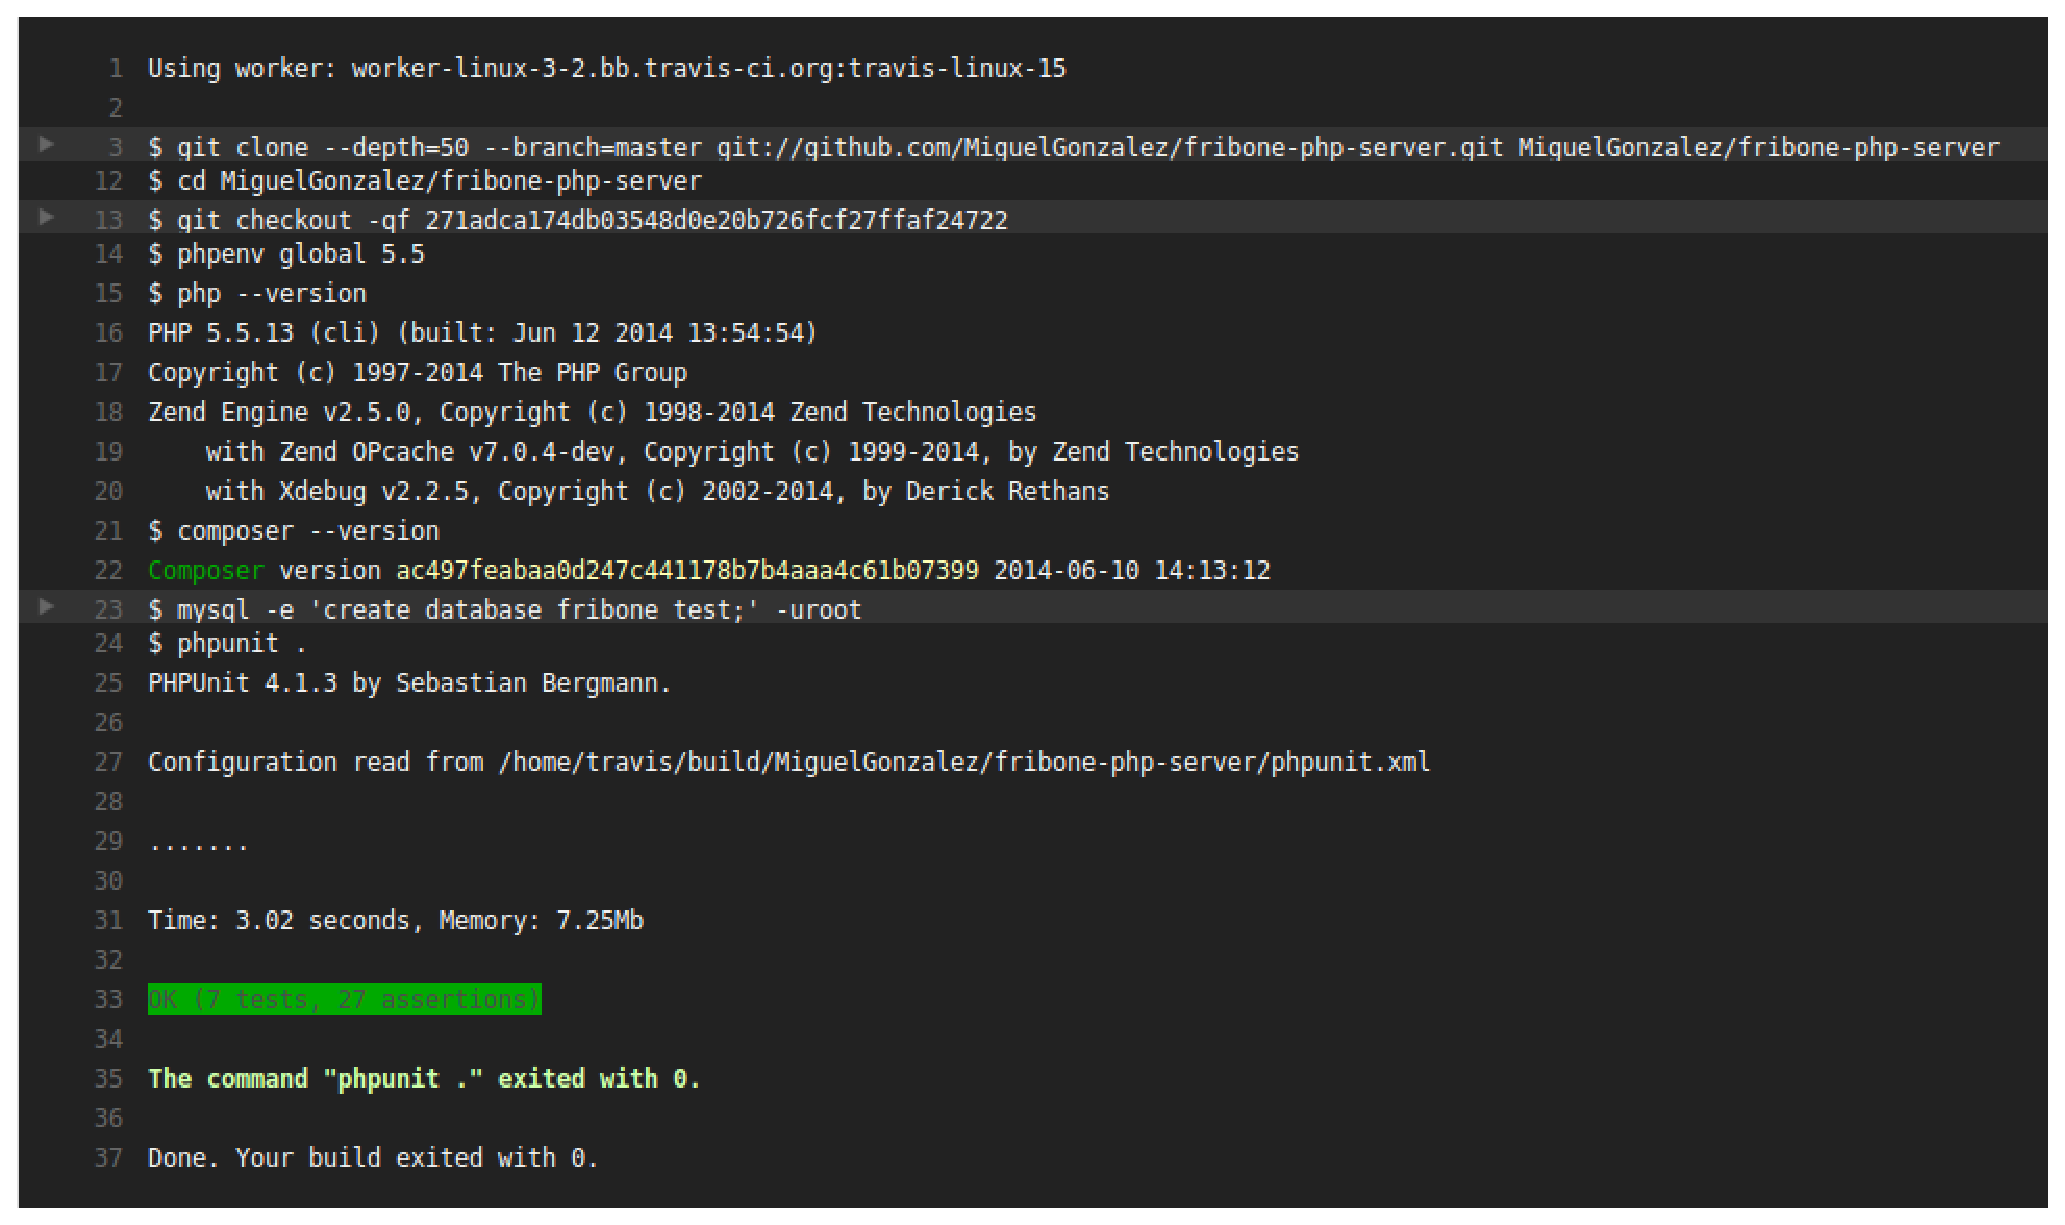
\includegraphics[keepaspectratio,width=0.9\textwidth]{travis-ci-tests.eps}
    \caption{Tets - Travis CI}\label{fig:travis-ci-tests}
\end{figure}

\subsection{Problemáticas para la creación de tests unitarios}

CodeIgniter viene con su propia herramienta para generar tests unitarios, la cual no nos permite su integración con \emph{Travis CI}, por ello se han realizado una serie de modificaciones para permitir el uso de PHPUnit.

Se han tenido que tocar los siguientes módulos y realizar los siguientes cambios:

\begin{itemize}

    \item Modificación del fichero \emph{DB\_driver.php}

        Si se produce un error se llama al método display\_error, el cual lo imprime por pantalla. Para correr tests se ha modificado para lanzar una excepción en caso de que se esté en el entorno de testing.

                \begin{lstlisting}
if (defined('ENVIRONMENT') && ENVIRONMENT == 'testing') {
    $message = $error . ' ' . $swap;
    throw new Exception($message);
} else {
    ...
    ...
}
                \end{lstlisting}

    \item Modificación del fichero Utf8.php

        Se ha modificado la línea donde se declara la variable global \emph{\$CFG} por el siguiente código para evitar un error al lanzarse los tests:

                \begin{lstlisting}
//global $CFG; // Fix PhpUnit Error
$CFG =& load_class('Config', 'core');
                \end{lstlisting}

    \item Modificado fichero \emph{mysql\_driver.php} para evitar un error al utilizar la función \emph{mysql\_escape\_string}:

                \begin{lstlisting}
function escape_str($str, $like = FALSE) {
        if (is_array($str)) {
            foreach ($str as $key => $val) {
                $str[$key] = $this->escape_str($val, $like); }

            return $str;
        }

        $str = is_resource($this->conn_id) ? mysql_real_escape_string($str, $this->conn_id) : addslashes($str);

        // escape LIKE condition wildcards
        if ($like === TRUE) {
            return str\_replace(
                array($this->_like_escape_chr, '%', '_'),
                array($this->_like_escape_chr.$this->_like_escape_chr,
                    $this->_like_escape_chr.'%', $this->_like_escape_chr.'_'),
                $str);
        }

        return $str;
    }
                \end{lstlisting}

\end{itemize}

Por último, para ser capaces de lanzar los tests se han tenido que añadir las siguientes configuraciones a la aplicación:

\begin{itemize}
    \item Creación del fichero de configuración \emph{phpunit.xml}

        Este fichero XML permite indicarle a PHPUnit los parámetros para ejecutar los tests. Consta de la siguiente configuración:

                \begin{lstlisting}
<?xml version="1.0" encoding="UTF-8" ?>
<phpunit bootstrap="application/application/tests/bootstrap.php"
    colors="true"
    convertErrorsToExceptions="true"
    convertNoticesToExceptions="true"
    convertWarningsToExceptions="true"
    processIsolation="false"
    stopOnFailure="false"
    syntaxCheck="false"
    verbose="true">
    <testsuites>
        <testsuite name="TestUserModel">
            <file>application/application/tests/models/UserTest.php</file>
        </testsuite>
        <testsuite name="TestLectorModel">
            <file>application/application/tests/models/LectorTest.php</file>
        </testsuite>
        <testsuite name="TestFridgeModel">
            <file>application/application/tests/models/FridgeTest.php</file>
        </testsuite>
        <testsuite name="TestSupermercadoModel">
            <file>application/application/tests/models/SupermercadoTest.php</file>
        </testsuite>
        <testsuite name="TestCompraModel">
            <file>application/application/tests/models/CompraTest.php</file>
        </testsuite>
        <testsuite name="TestLogin_auth">
            <file>application/application/tests/libraries/Login_authTest.php</file>
        </testsuite>
        <testsuite name="TestMy_PHPMailer">
            <file>application/application/tests/libraries/My_PHPMailerTest.php</file>
        </testsuite>
        <testsuite name="TestLector_library">
            <file>application/application/tests/libraries/Lector_libraryTest.php</file>
        </testsuite>
        <testsuite name="TestSupermercado_library">
            <file>application/application/tests/libraries/Supermercado_libraryTest.php</file>
        </testsuite>
        <testsuite name="TestFridge_library">
            <file>application/application/tests/libraries/Fridge_libraryTest.php</file>
        </testsuite>
        <testsuite name="TestCompra_library">
            <file>application/application/tests/libraries/Compra_libraryTest.php</file>
        </testsuite>
    </testsuites>
     <filter>
        <blacklist>
            <directory suffix=".php">application/application/config</directory>
            <directory suffix=".php">application/application/controllers</directory>
            <directory suffix=".php">application/application/core</directory>
            <directory suffix=".php">application/application/libraries/PHPMailer</directory>
            <directory suffix=".php">application/application/tests/mockups</directory>
            <directory suffix=".php">application/system</directory>
            <file>application/application/tests/bootstrap.php</file>
            <file>application/application/tests/database_inflater.php</file>
            <file>application/application/tests/PHPTest_Unit.php</file>
        </blacklist>
    </filter>
    <php>
        <const name="PHPUNIT_TEST" value="1" />
        <const name="PHPUNIT_CHARSET" value="UTF-8" />
        <const name="REMOTE_ADDR" value="217.0.0.1" />
    </php>
    <logging>
        <log type="coverage-text" target="php://stdout" showUncoveredFiles="true"/>
        <log type="coverage-clover" target="coverage/clover.xml"/>
    </logging>
</phpunit>
                \end{lstlisting}

        Ejecutará la aplicación a partir del fichero \emph{bootstrap.php} y lanzará los tests definidos.

    \item Creación del fichero \emph{bootstrap.php}

        Este fichero es una copia del \emph{index.php}, se ha modificado el entorno a testing, la dirección remota del servidor, el reporte de errores del sistema y el path de las carpetas:
                \begin{lstlisting}
define('ENVIRONMENT', 'testing');

$_SERVER["REMOTE_ADDR"]     = array_key_exists( 'REMOTE_ADDR', $_SERVER) ? $_SERVER['REMOTE_ADDR'] : '127.0.0.1';

error_reporting(E_ALL ^ E_NOTICE);
$system_path = '../../system';
$application_folder = '../../application';
                \end{lstlisting}

    \item En la definición de controlador global se ha añadido una condición para comprobar si se está en modo testing. En modo testing no se carga ninguna librería y se añade en su lugar la carpeta de \emph{tests/mockups} como paquete, de esta manera se cargarán automáticamente primero las librerías que se encuentren ahí por defecto, facilitando la creación de \emph{mockups} en el entorno de test.

                \begin{lstlisting}
if (defined('ENVIRONMENT') && ENVIRONMENT == 'testing') {
    $this->load->add_package_path(APPPATH.'tests/mockups');
} else {
    $this->load->library('login_auth');
}
                \end{lstlisting}
\end{itemize}

\subsection{Esquema de la base de datos}

    A continuación se muestra el esquema de la base de datos donde se observan las relaciones que hay entre las distintas entidades. En su diseño se ha tenido en cuenta que hay dos partes diferenciadas que necesitan un punto de unión:

    \begin{itemize}
        \item Zona del usuario

            Un usuario tendrá sus propios frigríficos y productos asociados a él

        \item Zona comunitaria

            En la zona comunitaria se crearán los supermercados y productos asociados a cada uno. Así, un usuario agregará a su frigoríficos los productos que de forma colaborativa se han guardado en la plataforma.

        \item Punto de unión

            La tabla \emph{my\_compra\_producto} enlaza entre un producto agregado por un usuario a una compra, al supermercado al que pertenece ese producto y que producto del supermercado es.

            Además, en esta tabla, se duplican todos los datos del producto del supermercado. De esta manera, se puede editar el precio del producto del supermercado y para un usuario; para tal compra; ese precio se mantiene.
    \end{itemize}

\begin{figure}[H]
    \centering
    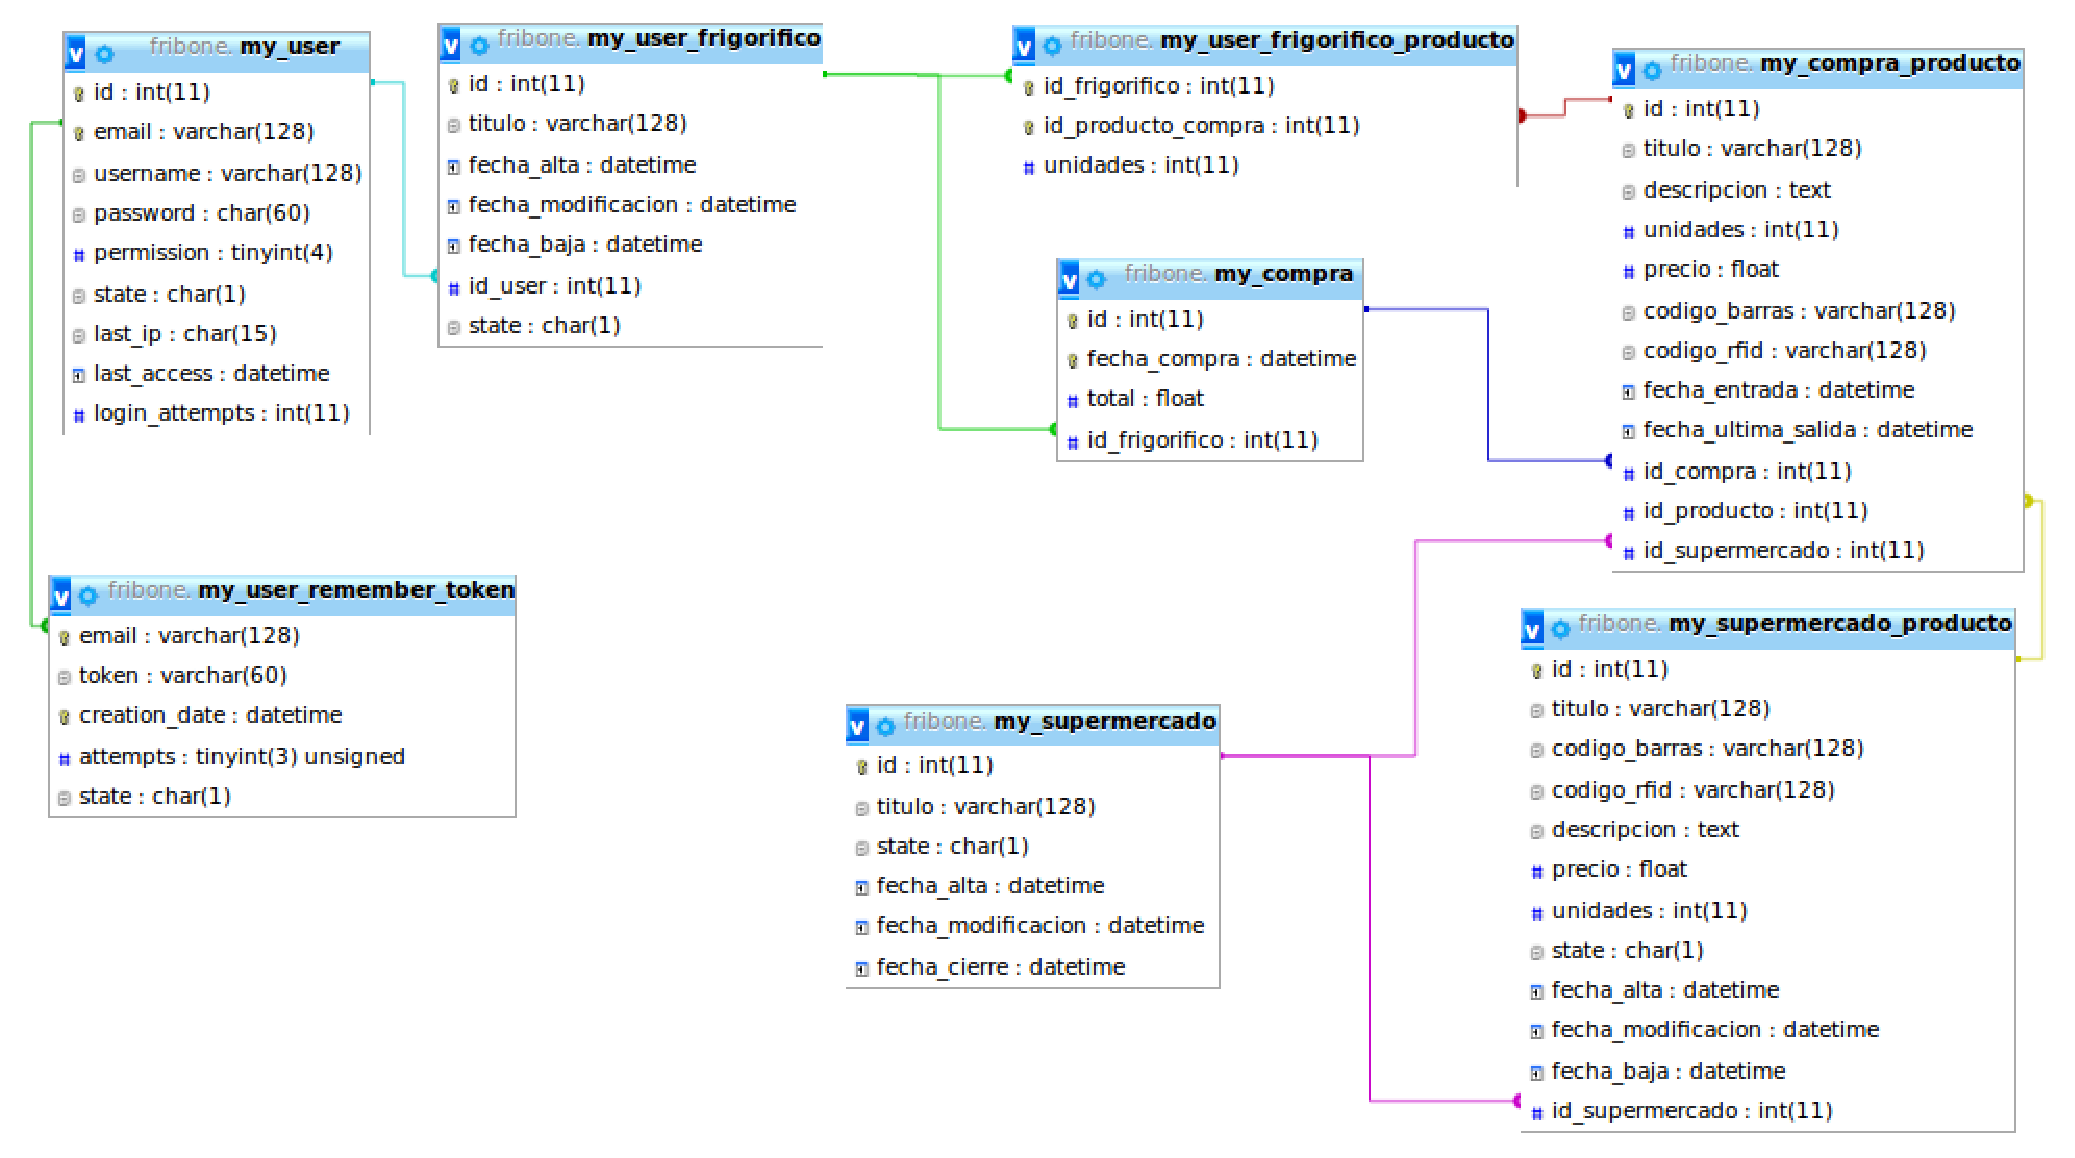
\includegraphics[keepaspectratio,width=0.9\textwidth]{esquema-bd.eps}
    \caption{Esquema de la base de datos}\label{fig:esquema-bd}
\end{figure}


\subsection{Esquema del servidor}

    El esquema de servidor se basa en el patrón \emph{MVC} (Modelo, Vista, Controlador) que provee \emph{CodeIgniter} con su framework.

    El modo de funcionar este patrón es el siguiente:

        \begin{itemize}
            \item Un usuario lanza una petición contra la siguiente url

                http://www.example.com/clientes/get\_cliente/1

            \item A través del modulo mod\_rewrite se redirige la petición al fichero \emph{index.php} de CodeIgniter, el cual se encarga de analizar la petición siguiendo el siguiente flujo de trabajo:

            \begin{figure}[H]
                \centering
                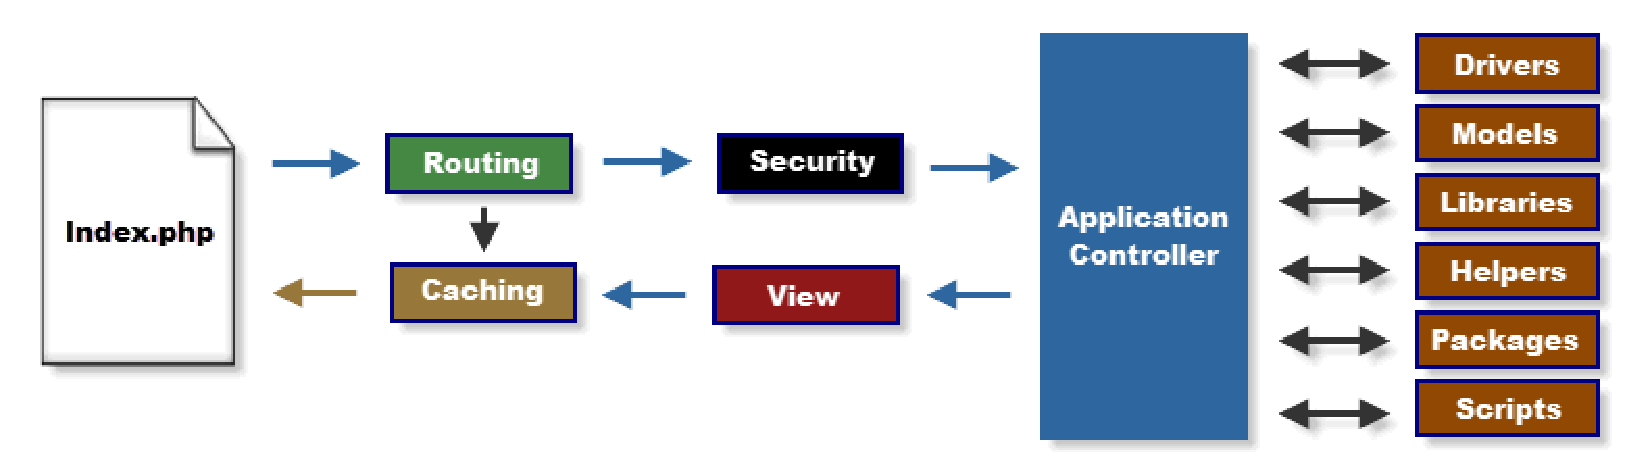
\includegraphics[keepaspectratio,width=0.9\textwidth]{flujo-trabajo-codeigniter.eps}
                \caption{Flujo de trabajo de CodeIgniter}\label{fig:flujo-trabajo-codeigniter}
            \end{figure}

            \item CodeIgniter descompone la URL en la siguiente estructura para conocer a que controlador tiene que pasar la petición, a que función llamar y qué parametros debe pasar.

                http://example.com/[controller-class]/[controller-method]/[arguments]

            Siendo para nuestro ejemplo los siguientes valores:

                \begin{itemize}
                    \item Controller class: clientes
                    \item Controller method: get\_cliente
                    \item Arguments: 1
                \end{itemize}
        \end{itemize}

    Los controladores son los encargados de procesar la petición, cargar tantas librerías, modelos... como necesiten para finalmente devolver un resultado.

    \subsubsection{Extendiendo el core de CodeIgniter}

    CodeIgniter al cargarse intenta buscar los sisguientes ficheros de sistema en la carpeta \emph{application/core}, esta funcionalidad permite sobreescribir algunas de las funcionalidades para ampliarlas.

    En el proyecto se han creado dos nuevos controladores para ampliar la funcionalidad del controlador por defecto de CodeIgniter:

    \begin{itemize}
        \item MY\_Controller

        Extiende de \emph{CI\_Controller} y se encarga de:

            \begin{itemize}
                \item Cargar la librería \emph{login\_auth} si no se están ejecutando los tests unitarios
                \item Ofrecer los siguientes métodos para renderizar la respuesta (\emph{\_renderJson}, \emph{\_renderXml}, \emph{\_renderToVar}, \emph{\_render})
            \end{itemize}

        \item MY\_Controller\_User

        Extiende de \emph{MY\_Controller} y únicamente se encarga de validar en el constructor que el usuario está logueado en el sistema, en caso de no estarlo, redirije a la Home pública.
    \end{itemize}

    \subsubsection{Esquema de controladores, modelos y librerías}

\subsection{Generación de código de barras}

Para enlazar el lector con la aplicación se generan dos códigos de barras que deben ser escaneador por el lector. Se ha ideado esta forma debido a que es la forma más sencilla que se tiene para introducir información en el aparato.

Para generar los códigos de barra se ha buscado una librería que cumpla con la codificación EAN-13 (\emph{European Article Number} ó \emph{International Article Number}). Es un sistema de codificación adoptado por más de 100 países compuesto por 13 dígitos que siguen el siguiente formato:

    \begin{itemize}
        \item Código del país (3 dígitos)
        \item Código de empresa (4 o 5 dígitos)
        \item Código del producto (completa los 12 primeros dígitos)
        \item Dígito de control
    \end{itemize}

Tras realizar una búsqueda de las librerías existentes en \emph{PHP} que cumplan estos requisitos, finalmente, se ha encontrado un proyecto en \emph{GitHub} (\url{https://github.com/rlt3/php-barcode}) que encaja con lo que se busca.

En la integración con el proyecto, como es de esperar en cualquier integración, se ha tenido un problema con el renderizado de los caracteres ya que utiliza una fuente que no estaba instalada en el sistema, como solución se ha añadido la fuente \emph{FreeSansBold.ttf} a la librería y se carga indicando la ruta a la fuente, así no se depende de la configuración del servidor. Además, se ha realizado un refactor de algunas de las funciones de la librería.

Una vez resueltos los problemas se ha realizado un \emph{Fork} de la librería, dejando los cambios refactorizados accesibles para futuros usos de la librería ó para cualquier otro usuario que realice una búsqueda de la misma.

A continuación se muestra el código para imprimir por pantalla un código de barras:

    \begin{lstlisting}
public function generar_barcode($number) {
    $barCode = new Barcode($number);
    $barCode->display();
}
    \end{lstlisting}